
\chapter{The JVML Back End}
\label{ch-jvm}

The Java Virtual Machine Language (JVML) back end was written as 
an experiment in translating machine code to run in a Java Virtual 
Machine (JVM).  There were 3 different versions of this back end. 
The original 1999 back end, \texttt{jbmu}, was a hand-written back end 
that supported translations of \hrtl\ onto JVML (i.e. Java bytecodes).
The \texttt{jbmu} translator was an experimental translator at best, 
to try and show the feasibility of translating to JVML.  The 
generated code would then be assembled by the Jasmin assembler. 
This translator is described in Section~\ref{sec-jbmu}. 

Realizing that so many of the optimizations that were needed in 
the \texttt{jbmu} translator were the same ones implemented by 
any optimizer such as the \texttt{gcc} compiler, Trent took over 
the job of writing a machine description (MD) file for the JVML 
language so that \texttt{gcc} could translated our low-level C 
code into JVML code, assembled by the Jasmin assembler. This 
work was done in 1999 and is described in Section~\ref{sec-gccjvm}.
The standalone \texttt{gcc} extensions to support JVML have been 
released under GPL and are not part of the distribution of the 
\uqbt\ system.  
 
In mid 2000, Sameer rewrote part of the JVML back end in Java, basically, 
making it similar in nature to the original \texttt{jbmu} back end.  
Brian extended this back end throughout the end of 2000, adding 
floating point support, non 32-bit integer types, type and size 
conversions, and more.  This translator is part of the 
\uqbt\ distribution, unfortunately, there is not much documentation 
for it at present time; we have put together some notes in 
Section~\ref{sec-jvmbackend}. 


\section{jbmu - A JVM Backend}
\label{sec-jbmu}

{\small
\begin{flushright}
Design: Trent and Cristina, Implementation: Trent, Documentation: Trent
[Mar 99]
\end{flushright}
}

This section describes the initial implementation of a JVM backend, 
jbmu, which was written in Java (Dec98-Feb99).  \uqbt 's intermediate 
representation was in fluctuation at the time, so the backend is 
dependent on an older version of \uqbt.  This backend was not completed; 
a second JVM backend was written for gcc.  
This documentation was written at a time when experimentation
with other stack-based languages was expected, as such, it
was designed to be retargetable.  
This chapter is left herein for historical reasons.  [Cristina - May 00]. 

The binary translation of an arbitrary source machine binary to stack
based machine bytecodes requires a generic frontend to produce non-machine
specific intermediate data and an efficient backend to produce target byte
codes.  To date, little work has been focused on the construction of
backends, especially for backends targeted at stack based machines.  
Current technologies in retargetable backends lend little to this task,
because they have taken the stance of Register Transfer Lists (RTLs) as an
intermediate representation.  This reduces the performance of target
machines that have less registers than source machines and fails to
address more serious needs of a stack based machine backend.  Other forms
of intermediate representation have been presented~\cite{Peyt99} but, to
date, RTLs appear the most recognised. The Java Virtual Machine, for
example, has no registers, however, the JVM specification allows any
method to use a defined number of local variables, which can be mapped
directly onto the integer registers of a source machine.  With these
problems in mind, we can state the task of the backend:

\begin{itemize}
\item To generate an internal representation.
\item To optimise that representation using non-machine specific
optimisations.
\item To perform generic stack based machine optimisations.
\item To generate bytecodes for a specific stack based machine.
\end{itemize}

The points above are well understood and their implementation can be seen
in compiler design but, despite this, there is little code that can be
reused in such a backend.  For this reason, it would be beneficial to
write a generic global optimiser that could be reused in other projects
and targeted at other machines.

\subsection{Non-Machine Specific Optimisations}

Non-machine specific optimisations can be done with no knowledge of the
target machine.  They are non-machine specific optimisations and, although
they sometimes can be improved with machine specific information, they are
generic and should be implemented with no knowledge of the target machine.  
This allows for the reuse of such code when retargeting to a different
machine.

The crucial stage of any backend is global optimisation.  Whatever the
internal representation, there is need for some basic optimisations:

\begin{itemize} 
\item Data flow analysis:  the movement of dead variable
values into sub-expressions.  This is particularly necessary in the case
of register-based machines to stack-based machines translation to
eliminate temporary register assignments.  This reduces the number of
``local variables'' a method requires which speeds up the overall code.

\item Constant folding:  any computation that can be done at compile time
is removed from the internal representation.  This leads to smaller
bytecode and less operations to be performed by the stack based
machine.

\item Common sub-expression elimination:  the availability of local
variables allows us to create temporaries for commonly used expressions.  
This prevents the re-computation of intensive expressions and reduces the
overall bytecode size.

\item Invariant movement and other optimisations:  more compiler
originated optimisations can be made by generating a control flow graph in
the internal representation and moving code.  This will result in faster
``inner loops'' and allow more opportunity for global optimisations like
constant folding. See~\cite{Aho86a} or~\cite{Fisc88b} for details.

\end{itemize}

\subsubsection{Bytecode Generation and Scheduling}

Every backend must eventually produce code for a specific target machine.  
This will inevitably lead to bytecode selection.  The instruction set of a
target machine may be redundant.  Often there is more than one way to
perform a series of operations with some being more efficent than others.
There are two primary solutions to this problem.  A compiler designer may
only use a subset of the available instructions, which leads to
inefficient code, or may attempt to choose the ``best'' instruction to
match the internal representation.

There is a lot of work on the subject and will not be
repeated here (for example, \cite{Emme88} speaks of a generic pattern
matching approach which may be useful, however, most of their code is in
Modula 2 and, as such, cannot be easily reused). Stack based machines
introduce more problems as the types of the operands must match the 
instruction generated.  This typing is to be considered extreme 
distinguishing between \texttt{char}, \texttt{int} and \texttt{byte} types.

The scheduling of instructions is most important on a stack-based machine.  
This can reduce the number of local variables used and, as a result, the
number of bytecodes need to store and retrieve them.  This is an obvious
job for dataflow analysis when the local variable is a temporary, but many
times the assignment of a local variable that is used at some later stage
can be replaced with an instruction that duplicates the value on the stack
at the appropriate moment.  These are topics that promise to give the most
optimisations in stack-based machine code.


\subsection{Internal Representations}

The retargetable stack based machine backend consists of a number of 
steps (figure ~\ref{fig-sbmbflow}):

\centerfigbegin
\resizebox{8cm}{!}
{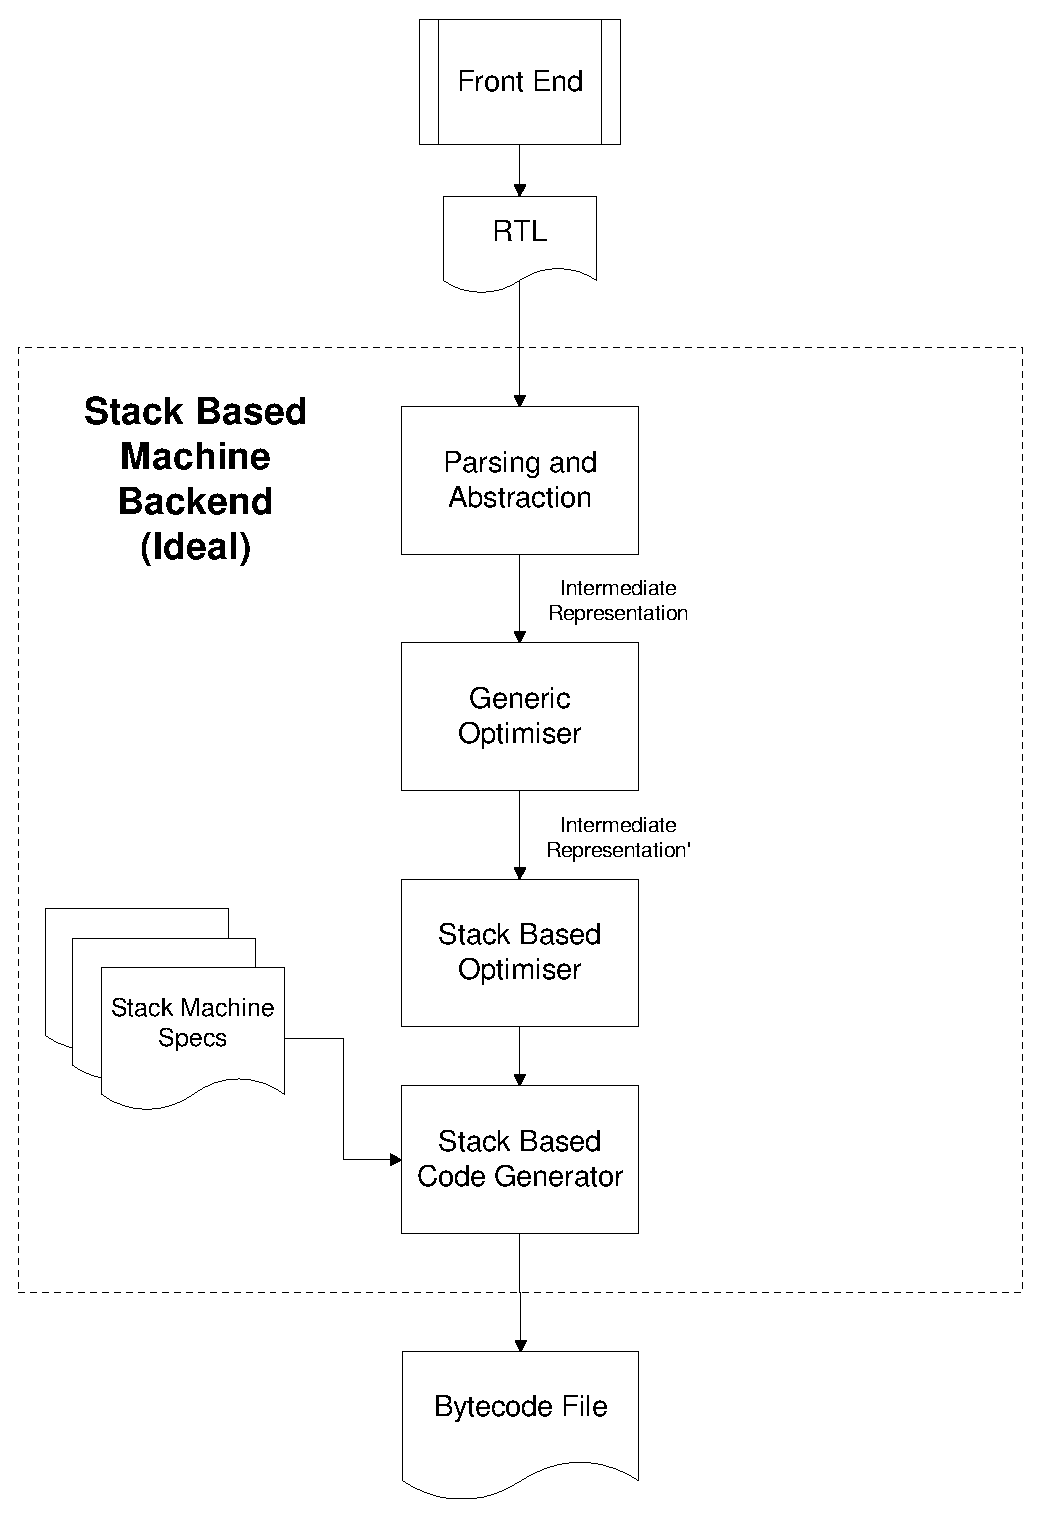
\includegraphics{figures/sbmbflow.eps}}
\centerfigend{fig-sbmbflow}{Flow Chart of the Stack Based Machine Backend}

\begin{enumerate}
\item Parsing and abstraction:  reduction of register transfer list
representation to basic assignment, call and branch statements.
\item Generic optimiser:  machine independant optimisation of those
statements.
\item Stack based optimiser:  stack based machine specific optimisations.
\item Stack based code generator:  generation of translated bytecodes
from the output of previous steps.  In the idealised model, the stack
based code generator can take a number of specification files that define
the target stack based machine.
\end{enumerate}

Each of these stages has an interface that interconnects them.  The
interface generated from parsing and abstraction of the RTL is used in the
optimiser.  This interface is known as the ``intermediate representation''
and consists of a control flow graph with each basic block containing an
array of statements.  The optimisers generate the same interface as they
receive, and as such, can be removed from the process when optimisations
are not required (such as in testing).  The code generator extends the
interface output from the optimiser with bytecode information placed in
each of the statements contained within a basic block. This data is then
linearised into an output file for the required machine.

The process depicted in figure ~\ref{fig-sbmbflow} is an idealisation of
the current experimental model of the stack based machine backend.  The
current process is better depicted in figure ~\ref{fig-sbmbflowcur} with
the difference being the final stage of processing.  Currently, the stack
based machine backend is targeted at the Java Virtual Machine and will be
hand extended to other stack based machines by rewritting this final
stage.  Once this is done, it will be easier to generalise about stack
based machines and approach the prefered model of absolute
retargetability.

\centerfigbegin
\resizebox{8cm}{!}
{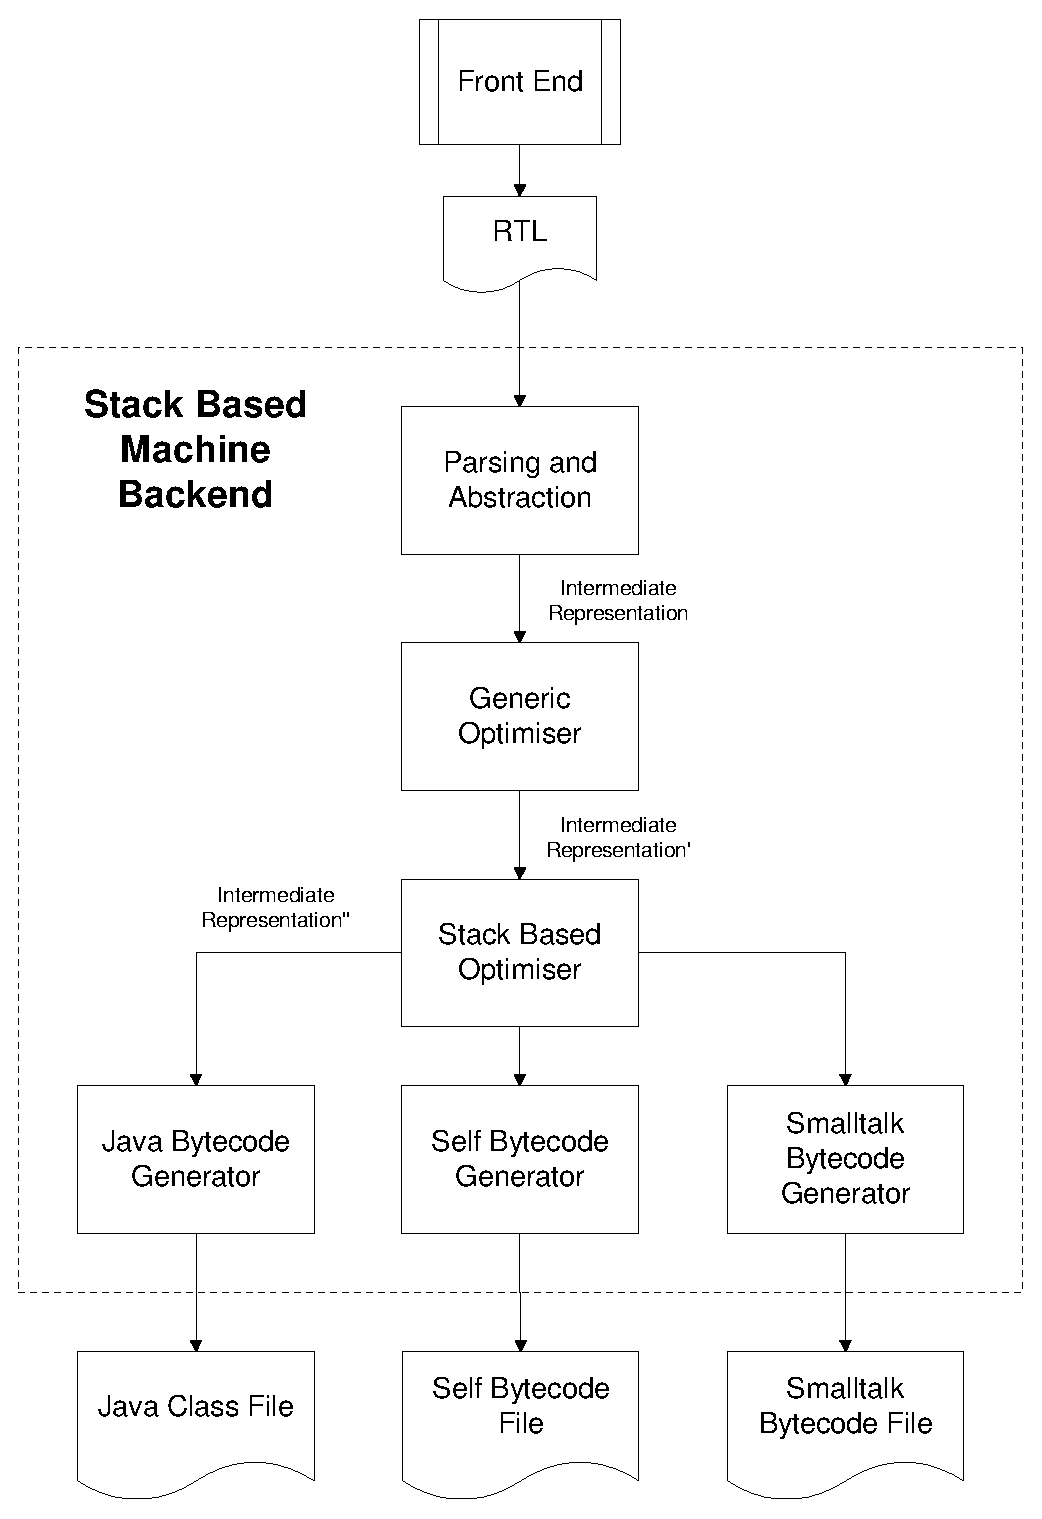
\includegraphics{figures/sbmbflowcur.eps}}
\centerfigend{fig-sbmbflowcur}{Experimental flow chart of the Stack Based Machine Backend}

\subsubsection{Intermediate Representation}

The intermediate representation consists of a control flow graph, that is,
a set of interconnected ``basic blocks''.  A basic block is defined as
having only one entry point and one exit point.  As control flows through
a program it follows a path that can be plotted.  If one was to plot all
the possible paths through a program, one would be constructing a control
flow graph.  In this way, a frontend programmer can use any form of
control structures in their language without fear of having to implement
them in the backend.  For example, an \texttt{if-then-else} structure
consists of four basic blocks.  The first basic block contains the
expression being tested.  If the expression is true, control flows to the
second basic block.  If the expression is false, control flows to the
third basic block.  Both the second and the third basic blocks fall
through to the fourth basic block.

\centerfigbegin
\resizebox{3cm}{!}
{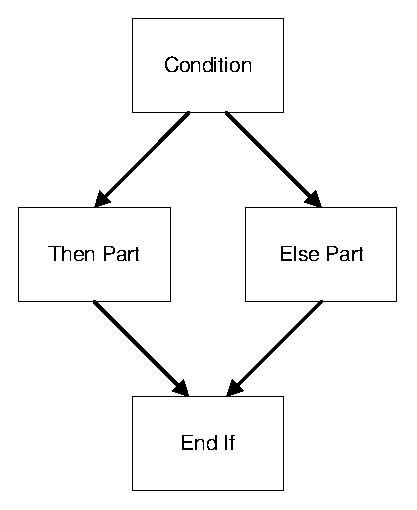
\includegraphics{figures/ifthenelse.eps}}
\centerfigend{fig-ifthenelse}{Control Flow Graph of an If-Then-Else
construct}

The first basic block is said to have two out-edges. The fourth basic
block has two in-edges.  A pretested loop is constructed just as easily.

Each basic block in the control flow graph contains an array of
statements.  These statements are mainly assignment statements but some
are also call statements.  Basic blocks which have two out edges (called
``two-ways'') have an extra statement attached, the ``conditional
statement''.  Statements are made up of expressions.  An expression can be
many things including arithmetic operations, logical operations, call and
assignment operations.  Each expression may have a number of parameters.
Expressions with two parameters are the binary expressions (add, multiply,
divide, etc).  Expressions with one parameter are the unary expressions
(negate, not, etc).  Unary expressions store their one parameter in the
``left'' node whereas binary expressions use both the ``left'' and
``right'' nodes.

These parameters are used to construct a tree structure for each
statement.  An optimiser will walk this tree structure and perform
optimisations that modify the structure.  A code generator will walk the
tree structure and generate code to be placed in various nodes of the
tree.  Both these uses of the tree structure require additional
information to be added to various nodes.  Specifying this data in the
intermediate representation classes would be non-generic and may result in
bloated trees filled with data that never gets used.  This method would
also mean that the intermediate representation would have to be changed
with every new use of the structure.  One would have to be very careful to
not ``break'' the data structure by removing anything that a user of a
previous version of the data structure may have assumed would never
change.  A solution to this problem is to allow the extension of
``objects'', that is, the instantiation of classes, not just classes
themselves.  To do this, each Java class in the implementation of the
intermediate representation is defined as an extension of the
``Extendable'' class.  A method can now be written to extend any of these
classes in such things as an optimiser or a code generator.

\subsubsection*{Data structure of the intermediate representation}

The Intermediate Representation contains a number of classes that
form a hierarchical structure of usage:
\begin{description}
\item [Program] is used to represent a complete program.  It contains an
array of procedures.
\item [Procedure] is used to represent a single procedure.  It contains
the name of the procedure and a control flow graph.
\item [BasicBlock] is used to construct a control flow graph.  It contains
a type, an array of in-edges, an array of out-edges, and an array of
statements.  Basic blocks of the \texttt{twoway} type contain a
\texttt{condition statement} which is used to determine which of the two
out-edges are followed during program execution.
\item [Expression] is used to construct statements.  Expressions contain a
type, a single integer parameter, and left and right expressions depending
on the expression type.  \texttt{Call} expressions contain an array of
expressions that are the parameters to the call.
\end{description}

\subsection{Examples}

The following examples show the current state of the UQBT frontend and the
stack based machine backend.  The following C program tests
assignments and simple conditional branches.  It is written on the SPARC 
archetecture:
\begin{verbatim}
void main() {
int i,j,k;

  j = i+k;
  k=6;
  i=j+5;

  printf("%i\n",i);
  if (j<k) 
    printf("%i\n",j);
  printf("%i\n",k);

}
\end{verbatim}
UQBT generates an output file which is parsed by the stack based machine
backend into the following statements in the intermediate representation.
\begin{verbatim}
proc main

bb type call
r[8] := r[48] 
r[9] := r[50] 
r[8] := r[8] + r[9] 
r[49] := r[8] 
r[8] := 0 | 6 
r[50] := r[8] 
r[8] := r[49] 
r[9] := r[8] + 5 
r[48] := r[9] 
r[9] := 69 << 10 
r[8] := r[9] | 552 
r[9] := r[48] 
Call printf(r[8],r[9])  

bb type twoway
r[8] := r[49] 
r[9] := r[50] 
r[0] := r[8] - r[9] 
bb cond: r[0] >= 0 

bb type call
r[9] := 69 << 10 
r[8] := r[9] | 552 
r[9] := r[50] 
Call printf(r[8],r[9])  

bb type call
r[9] := 69 << 10 
r[8] := r[9] | 552 
r[9] := r[49] 
Call printf(r[8],r[9])  

bb type ret
\end{verbatim}
These statements are passed to the code generator for Java, which adds
bytecode information to each of the nodes in the Intermediate 
Representation. Note that optimisation has been disabled for this example.  
The Intermediate Representation is then flattened to produce an output
file.  Comments have been added for clarity:
\begin{verbatim}
L0:
        iload 48        ; r[8]  := r[48]
        istore 8
        iload 50        ; r[9]  := r[50]
        istore 9
        iload 8         ; r[8]  := r[8] + r[9]
        iload 9
        iadd
        istore 8
        iload 8	        ; r[49] := r[8]
        istore 49
        ldc 0           ; r[8]  := 0 | 6
        ldc 6
        ior
        istore 8
        iload 8         ; r[50] := r[8]
        istore 50
        iload 49        ; r[8]  := r[49]
        istore 8
        iload 8         ; r[9]  := r[8] + 5
        ldc 5
        iadd
        istore 9
        iload 9         ; r[48] := r[9]
        istore 48
        ldc 69          ; r[9]  := 69 << 10
        ldc 10
        ishl
        istore 9
        iload 9         ; r[8]  := r[9] | 552
        ldc 552
        ior
        istore 8
        iload 48        ; r[9]  := r[48]
        istore 9
        iload 8         ; Call  printf(r[8],r[9])
        iload 9
        invokestatic printf
        goto L1

L1:
        iload 49        ; r[8]  := r[49]
        istore 8
        iload 50        ; r[9]  := r[50]
        istore 9
        iload 8         ; r[0]  := r[8] - r[9]
        iload 9
        isub
        istore 0
        iload 0         ; bb cond: r[0] >= 0
        ldc 0
        if_icmplt L2
        goto L3

L2:
        ldc 69          ; r[9]  := 69 << 10
        ldc 10
        ishl
        istore 9
        iload 9         ; r[8]  := r[9] | 552
        ldc 552
        ior
        istore 8
        iload 50        ; r[9]  := r[50]
        istore 9
        iload 8         ; Call  printf(r[8],r[9])
        iload 9
        invokestatic printf
        goto L4

L3:
        ldc 69          ; r[9]  := 69 << 10
        ldc 10
        ishl
        istore 9
        iload 9         ; r[8]  := r[9] | 552
        ldc 552
        ior
        istore 8
        iload 48        ; r[9]  := r[49]
        istore 9
        iload 8         ; Call  printf(r[8],r[9])
        iload 9
        invokestatic printf
        goto L2

L4:
        ret

\end{verbatim}
This bytecode is unoptimised which is to be expected as the Intermediate
Representation is unoptimised.  The generic optimiser reduces the number
of statements in the intermediate representation.  The stack based 
machine optimiser uses specific stack based machine optimisations to
reduce the number of bytecodes, local variables and stack depth.  Finally,
the code generator for the Java Virtual Machine selects the best bytecodes
to be used in the final output.

\subsection{The Runtime Environment}

Binary translation is not just a compiler backend (though it can be).  
Generally, there is a lot of code that can be shared between translated
programs.  This code has the task of emulating the environment that the
code was originally written for.  Such things as calling conventions and
dynamic linking must be known to the backend to generate code that can
link to its new environment.  We can see the need for a run time
environment through a case study.  The following C program:
\begin{verbatim} 
void main() {
  printf("hello world\n");
}
\end{verbatim}
compiles to the following assembly code (some code is removed for the
purpose of readability):

\begin{verbatim} 
.LLC0:
        .asciz  "hello world\n"

        sethi %hi(.LLC0),%o1
        or %o1,%lo(.LLC0),%o0
        call printf,0
        nop
        ret
\end{verbatim}

which can be translated and optimised to:
\begin{verbatim} 
        r[0] := .LLC0;
        call printf
        return 
\end{verbatim} 

Finally we can add to this
code the knowledge of calling convention.  On a SPARC, parameters are
passed in the first six general purpose integer registers.  The function
\texttt{printf} expects to see a pointer to an asciiz string as its first
parameter.  This is a problem in Java, for example, because \texttt{.LLC0}
refers to an offset in the source binary's read-only data section.  The
translated program will need access to this data if it is to pass the
string onto a function like \texttt{System.out.println}. The problem is
actually harder than that.  \texttt{System.out.println} expects a
\texttt{String} object type which is quite different to an asciiz string.  
The translated program will need to construct such an object using a
method not unlike the following:
\begin{verbatim} 
static String getstring(int rodatastart,byte[] rodata,int i) {
    String a = "";
      while (rodata[i-rodatastart]!=0) {
        a += (char)rodata[i-rodatastart];
        i++;
      }
      return a;
  }
\end{verbatim} 
The first parameter is the source machine address of the start of the
read-only data section.  The second parameter is a reference to the actual
bytes contained within the read-only data section.  The final parameter is
the source machine address of the asciiz string which we assume to be
located somewhere within the read-only data section.  We refer to this
calling structure as ``passing core'' and it must be used in all runtime
support libraries.

Finally the \texttt{printf} function must be written in Java to link with
the translated binary.  The function could be as simple as a wrapper to
the equivalent Java function or, in the case of printf, something more
complicated.  This must be done for every library function to be called.  
The size of a run-time environment is extensive in the case of graphical
user interface (GUI) environments.  This can be seen in the WINE
project~\cite{Wine96} which aims to emulate the Microsoft Windows
environment on 80x86 X-windows systems.  We can reuse most of the work in
that project.  This promotes the feasibility of binary translation of
Windows executables to the JVM with an interface to the awt classes.  The
biggest obstacle of the WINE project is the Application Binary Interface
(ABI) of Microsoft Windows.  Each binary refers to more than its own data
segments and system API calls.  In many operating systems, applications
have access to data structures stored in shared libraries and, as in the
case of Microsoft Windows, in the operating system itself.  These
references must be recognised by the backend and replaced with a reference
to the runtime support class.  These problems are not limited purely to
Microsoft Windows (although they appear most abundantly there), they also
pop up in SPARC binaries.  One such example is the use of \texttt{errno}
from the standard I/O C libraries.  \texttt{Errno} is a global integer
that resides in a shared library.  When it is written to, the page that is
shared is copied into the new process space.  One would wish a backend to
recognise global variables that reside in support libraries and redirect
them to the runtime support class.


\subsection{Summary}

The development of backends borrows heavily from the field of optimising
compilers.  The targeting of a backend to a stack based machine introduces
new problems in optimisation.  The JVM and its strict typing introduces
problems that have rarely been seen by compiler writers before.  A runtime
support library is necessary to minimize the size of the translated
applications and is specific to each source machine and platform.  The
development of a binary translator to Java bytecodes promises a new
mentality in application distribution.  The ``translate once, run
anywhere'' concept is already within our reach, what still awaits is a
resultant application that runs with a similar performance on the JVM as
on the source machine.  This work outlines the steps involved in such a
backend and takes the first tentative steps towards that end.



\section{gcc-jvm - A JVM Backend for the gcc Compiler} 
\label{sec-gccjvm}

{\small
\begin{flushright}
Design: Trent, Implementation: Trent, Documentation: Trent [Aug 99]
\end{flushright}
}

This section describes Trent's experiences with porting
EGCS (gcc version 1.1.2) to a stack-based machine, 
the JVM in particular.  It is written in first person.  

When I first began investigating the possibility of porting the
Experimental GNU Compilation Set (EGCS) to the Java Virtual Machine (JVM)
I thought it would be possible to semantically describe the JVM to EGCS
and have it adequately generate stack based machine byte codes.  I hoped
that I would be able to specify to the back end that the only way to load
a constant or a register (local variable) was via the stack and EGCS would
break its internal representation effectively.  This appears to be a
little too optimistic.  My attempts at constructing a machine description
where EGCS is forced to do all moves via the stack failed, not because I
was supplying too little information to the back end, but because I was
supplying too much.  This lead to an alternate strategy:  I decided to
take all the instructions that one would find on a register based machine
and implement them using a number of byte codes.  The resultant byte code
was a poor but correct representation of the original program.  Soon I had
simple programs (hello world) working and could actually perform some
benchmarks.  The results were astounding: small register transfer bound
programs ran at comparable speeds to native code.  This is best explained
with an example.

\begin{verbatim}
int fibo(int i) {
  if (i<2) return 1;
  else return fibo(i-1)+fibo(i-2);
}

void main(int argc,char **argv) {
  printf("fibo %i is %i\n",40,fibo(40)); 
}
\end{verbatim}

Fibonacci is a register transfer bound program that takes 22 seconds on a
SPARC Ultra 9 to run natively.  If we compile it to JVM byte code we get
the following (for the fibo function).

\begin{verbatim}
.method public _fibo(I)I
        .limit stack 9
        .limit locals 17
        
        iconst_0
        istore 14
        
        iload 1
        bipush 1      
        if_icmple L2
        
        iload 1  
        bipush -1
        iadd
        istore 10
        
        aload_0
        iload 10
        invokevirtual Fibo/_fibo(I)I
        istore 10   
        
        iload 10 
        istore 13
        iload 1  
        bipush -2
        iadd   
        istore 10
        
        aload_0     
        iload 10
        invokevirtual Fibo/_fibo(I)I
        istore 10
        
        iload 13 
        iload 10 
        iadd   
        istore 10
        
        goto L8     
L2:
        bipush 1
        istore 10

L8:
        iload 10 
        ireturn
.end method
\end{verbatim}

On the same machine running version 1.1 of the JVM, this bytecode takes
90 seconds to run.  The overhead is caused primarily by the two method
calls.  The following Java source code compiles to a program with the same
functionality.

\begin{verbatim}
class Fib {

  int fibo(int i) {
    if (i<2) return 1;
    else return fibo(i-1)+fibo(i-2);
  }

  void main(int argc,int argv) {                 
    System.out.println("fibo " + 40 + " is " + fibo(40));         
  }

  public static void main(String[] args) {
    Fib f = new Fib();
    f.main(0,0);
  }
}
\end{verbatim}

The resultant class file takes 56 seconds to run.  Significantly less than
the EGCS generated byte code.  The following is the byte code that is
generated by javac (for the fibo method above).

\begin{verbatim}
Method int fibo(int)
   0 iload_1
   1 iconst_2
   2 if_icmpge 7
   5 iconst_1
   6 ireturn
   7 aload_0
   8 iload_1
   9 iconst_1
  10 isub
  11 invokevirtual #13 <Method int fibo(int)>
  14 aload_0
  15 iload_1
  16 iconst_2
  17 isub
  18 invokevirtual #13 <Method int fibo(int)>
  21 iadd
  22 ireturn   
\end{verbatim}

Smaller size and less local variable usage improves the speed of the byte
code.  A possible solution to this problem is to use a post processing
optimisation stage such as BLOAT.  When applied to the poor byte code
generated by EGCS, it produces the following.

\begin{verbatim}
Method int _fibo(int)
   0 iload_1
   1 iconst_1
   2 if_icmple 31
   5 iload_1
   6 iconst_m1
   7 iadd
   8 istore_2
   9 aload_0
  10 iload_2
  11 invokevirtual #20 <Method int _fibo(int)>
  14 istore_2
  15 iinc 1 -2
  18 aload_0
  19 iload_1
  20 invokevirtual #20 <Method int _fibo(int)>
  23 istore_0
  24 iload_2
  25 iload_0
  26 iadd
  27 istore_0
  28 goto 33
  31 iconst_1
  32 istore_0
  33 iload_0
  34 ireturn
\end{verbatim}

This is still a lot more bytecodes than the javac generated output but
runs in 55 seconds.  This leads to an apparent paradox:  How can more 
bytecodes run faster than less byte codes?  The answer lies in the behaviour
of the Just In Time compiler.  For version 1.1 of the JVM one can export
an environment variable JIT\_ARGS to 'dump' to print excessive amounts of
debugging information.  Using the bash shell one would do the following
command:
\begin{verbatim}
		export JIT_ARGS=dump
\end{verbatim}

Now any execution of the JVM will result in JIT debugging information
being dumped to standard error.  For version 1.2 of the JVM one would do
the following command:
\begin{verbatim}
		export _JIT_ARGS=dump
\end{verbatim}

The following is output by the JIT for the javac generated bytecode:
\begin{verbatim}
     0 iload_1        1b     
     1 iconst_2       05           
     2 if_icmpge      a2 00 05
        subcc   %i1, 2, %g0
        bge     5
        nop     
     5 iconst_1       04     
     6 ireturn        ac
        or      %g0, 1, %i0
        ba      8
        nop        
     7 aload_0        2a           
     8 iload_1        1b     
     9 iconst_1       04
    10 isub           64   
        sub     %i1, 1, %l0           
    11 invokevirtual  b6 000d
        or      %l0, %g0, %o1
        or      %g0, %i0, %o0
        ld      [%o0 + 4], %g1
        ld      [%g1 + 52], %g1
        ld      [%g1 + 68], %g1
        jmpl    [%g1 + %g0], %o7
        nop
        unimp   0x000a5a78 
        or      %g0, %o0, %l0    
    14 aload_0        2a        
    15 iload_1        1b        
    16 iconst_2       05    
    17 isub           64
        sub     %i1, 2, %l1        
    18 invokevirtual  b6 00 0d
        or      %l1, %g0, %o1
        or      %g0, %i0, %o0
        ld      [%o0 + 4], %g1
        ld      [%g1 + 52], %g1
        ld      [%g1 + 68], %g1
        jmpl    [%g1 + %g0], %o7
        nop
        unimp   0x000a5a78 
        or      %g0, %o0, %l1    
    21 iadd           60
        add     %l0, %l1, %l0        
    22 ireturn        ac
        or      %g0, %l0, %i0
\end{verbatim}
  
The major overhead of the above code being the two method calls.  
Ignoring the method calls, ten native machine instructions are generated.  
The following is output for the BLOAT optimised EGCS output:
\begin{verbatim}
     0 iload_1        1b     
     1 iconst_1       04     
     2 if_icmple      a4 00 1d
        subcc   %i1, 1, %g0
        ble     5
        nop     
     5 iload_1        1b    
     6 iconst_m1      02
     7 iadd           60
        add     %i1, -1, %i2          
     8 istore_2       3d           
     9 aload_0        2a     
    10 iload_2        1c     
    11 invokevirtual  b6 0014
        or      %i2, %g0, %o1
        or      %g0, %i0, %o0 
        ld      [%o0 + 4], %g1
        ld      [%g1 + 200], %g1
        ld      [%g1 + 68], %g1
        jmpl    [%g1 + %g0], %o7
        nop
        unimp   0x000a5b60
        or      %g0, %o0, %l0
    14 istore_2       3d
        or      %g0, %l0, %i2         
    15 iinc           84 01fe   
        add     %i1, -2, %i1           
    18 aload_0        2a        
    19 iload_1        1b    
    20 invokevirtual  b6 0014
        or      %i1, %g0, %o1 
        or      %g0, %i0, %o0
        ld      [%o0 + 4], %g1  
        ld      [%g1 + 200], %g1
        ld      [%g1 + 68], %g1
        jmpl    [%g1 + %g0], %o7
        nop
        unimp   0x000a5b60
        or      %g0, %o0, %l0    
    23 istore_0       3b
        or      %g0, %l0, %i0        
    24 iload_2        1c        
    25 iload_0        1a           
    26 iadd           60  
        add     %i2, %i0, %i0    
    27 istore_0       3b        
    28 goto           a7 0005
        ba      1e
        nop    
    31 iconst_1       04
    32 istore_0       3b
        or      %g0, 1, %i0    
    33 iload_0        1a    
    34 ireturn        ac
\end{verbatim}

Again ignoring the two method calls, eleven native machine instructions
are generated.  One can now see that byte code size is not an entirely
fair measure of resultant JIT generated code size.

The introduction of local variable usage that cannot be mapped into
registers (for example, local arrays) a register based machine requires a
stack frame.  Commonly, a stack pointer and a frame pointer are maintained
to point to a section of volatile memory.  This posses a problem for the
JVM port: there is no generic memory.  Possible solutions are to maintain
a "stack" array of bytes and do all stack accesses to that array.  The
problem becomes more complex when one considers global memory.  The
solution I originally chose was to perform all memory input/output with a
method contained within a run time support class.  The method to read an
integer from any arbitrary point in memory was called memref and the
method to store an integer to any arbitrary point in memory was called
memstore.  These two methods would examine the address requested and
determine the required array reference: read only data, read/write data or
stack.  To perform a memory reference the backend need only generate the
following:
\begin{verbatim}
sipush 24324   ; address
invokevirtual Classname/memref(I)I
istore 9
\end{verbatim}

The resultant bytecode was very easy to read and could be easily debugged
(for example, one could monitor all reads and writes to memory).  
Unfortunately memory bound programs experienced dramatic performance
losses.  In the order of sixty times slower execution.  The solution was
to move all memory references inline and abandon the array segregation.  
All memory was placed in a single array, called "memory", in the run time
support class and now the back end is required to generate significantly
more code.  To load an integer from an unsigned byte array one need only
perform the following (big endian).

\begin{verbatim}
Register := memory[location] << 24 | 
    memory[location+1] << 16 | 
    memory[location+2] << 8 | 
    memory[location+3]
\end{verbatim}

However, the JVM does not have unsigned types, and thus each signed byte
must be converted to an integer representation of its unsigned value:
\begin{verbatim}
Register := (memory[location]<0?256+memory[location]:memory[location]) << 24 | 
    (memory[location+1]<0?256+memory[location+1]:memory[location]) << 16 | 
    (memory[location+2]<0?256+memory[location+2]:memory[location+2]) << 8 | 
    (memory[location+3]<0?256+memory[location+3]:memory[location+3])
\end{verbatim}

To improve the performance of each integer memory reference, the memory
array is made an array of int instead of an array of byte.  Initialised is
then put into the array already in unsigned format.  The speed increase
comes at the expense of a 4:1 increase in space requirements.  The
following code is generated by the back end to perform an integer memory
reference:
\begin{verbatim}
        aload_0
        getfield Classname/memory [I
        iload 12 ; address
        dup2  
        iaload  
        bipush 8
        ishl
        dup_x2
        pop 
        iconst_1
        iadd
        dup2
        iaload   
        bipush 16
        ishl    
        dup_x2  
        pop 
        iconst_1
        iadd
        dup2
        iaload
        bipush 8
        ishl     
        dup_x2   
        pop     
        iconst_1
        iadd
        iaload  
        ior 
        ior 
        ior
        istore 11  ; destination
\end{verbatim}

The same memory bound benchmarks now run at 20 to 30 times as slow.  
Memory management is still a significant issue that is difficult to
resolve.


\subsection*{The build process}

The output of the compiler proper is one jasmin~\cite{Meye97} 
assembler file per C language input file.  
If the input files contain no global data, the build
process is simple, concatenate the multiple jasmin files into a single
file and assemble to a class file.  However, C files containing global
data produce an addition output file global.s.  References to labels
contained in global.s will appear in the jasmin output preceded by
"symref" and proceeded by "end".  As each C input file is compiled, the
global.s outputs are concatenated together into gglobal.s.  This file is
assembled to object format and a search and replace program (sed) is used
to replace each symbol reference with an offset into the data section.  
Finally the object file is objcopied into a raw data file and passed to
the run time support class to be loaded into the memory array.  This
process is only needed in programs with multiple input files and global
data.


\section{The Java JVM Back end}
\label{sec-jvmbackend}

{\small
\begin{flushright}
Design: Cristina and Brian, Implementation: Sameer [Aug 00], Brian [Nov 00],  
	Documentation: Brian [Nov 01]
\end{flushright}
}

The Java JVM back end is a rewrite of the C-based original JVM 
back end that was written in early 1999.  We were interested in 
seeing whether the Java language could be used to write back ends 
for our translator needs.  The following notes explain part of the
operation of this back end. 
Experience with the user of this back end is described in the 
{\emph{Experience}} chapter (Chapter~\ref{ch-experience}) in 
Section~\ref{sec-to-jvm}.  

The Java JVM backend operates much like the C and other backends. 
Unlike the C (Chapter~\ref{ch-cbackend}) and the VPO (Chapter~\ref{ch-vpobackend}) 
backends, however, it is single-pass. The Jasmin code for each procedure is
emitted in one pass. A small runtime library implemented in the file
\texttt{TranslatedFile.java} provides support for the generated code. That 
file contains a method \texttt{realMain} that is called first when the 
translated program starts execution. The \texttt{realMain()} method 
initializes the memory used by the translated program and copies the program's 
command line arguments into that memory.  The \texttt{realMain()} method 
then calls the translated program's \texttt{\_main()} method, which contains 
the code for the program's main procedure. All generated methods are static 
except for \texttt{\_main()}. This is done for technical reasons 
(\texttt{\_main} is declared abstract in \texttt{TranslatedFile.java}).

It recursively processes a source procedure's HRTLs for a procedure and
emits directives for each HRTL into a Jasmin source file. Given a HRTL, it
checks first whether it is a high-level HRTL such as a CALL\_HRTL, or if it
is a RTLList, a list of low-level RTLs. If the former, directives for the
control transfer or other high-level HRTL are emitted. If the latter,
directives for each RTL in the list are emitted. A postorder traversal of
each RTL's subexpressions produces the stack-oriented JVM bytecodes for that
RTL. 

Memory is represented using a single large Java byte array "memory". The
source program's bss and data segments are read into the appropriate
elements of that array so that a data item at a particular
address x can be read from memory[x].

The most complex thing (perhaps) about the JVM backend's operation is its
allocation of JVM locals for the HRTL variables:

\begin{itemize} 
\item Local 0 always holds the Java \texttt{this} reference if the procedure 
	is \texttt{\_main()}, and the first procedure argument otherwise.
\item Locals 1-7: all or remaining formal parameters (assumes there are 
	up to 6 parameters at most).
\item Local  8 and 9: unused.
\item Local [10..(10+n)): the n local HRTL variables used in the method.
\item Locals [(10+n)..99]: the HRTL temporary registers.
\item Local 100: a temporary variable used for, e.g., byte swapping.
\end{itemize}


\subsection{Usage of the Java JVM Backend}
To use the JVM backend,
build \uqbt\ with \texttt{with-target=sparc}
and then request the JVM backend using the command line option \texttt{-j}.
This will make \uqbt use the JVM backend
rather than the default low-level \texttt{C} backend.
The \texttt{Makefile} generated in the output directory created by \uqbt\ 
includes rules to run Jasmin and build the necessary Java class files for
the translated program.


